\chapter{Work done}
After running a model with a fiducial set of parameters, we found that in the disk upper layer heating is dominated by photoelectric effect, followed by H2 formation heating in the photodissociation layer, and viscous heating in the deep region. Cooling is dominated by O i and C ii lines in the upper layer, and by accommodation on the dust grains in the lower dense layers. Overall the distribution of the dominant heating and cooling mechanisms is similar to what is shown in Woitke et al. (2009).
\begin{figure}[h]
	\centering
	\includegraphics[width=0.6\linewidth]{../../../Downloads/Screenshot_from_2023-08-31_23-17-04-removebg-preview}
	\caption{Flowchart depicting the working of the model}
	\label{fig:screenshotfrom2023-08-3123-17-04-removebg-preview}
\end{figure}

\section{Results}
\begin{figure}[h]
	\centering
	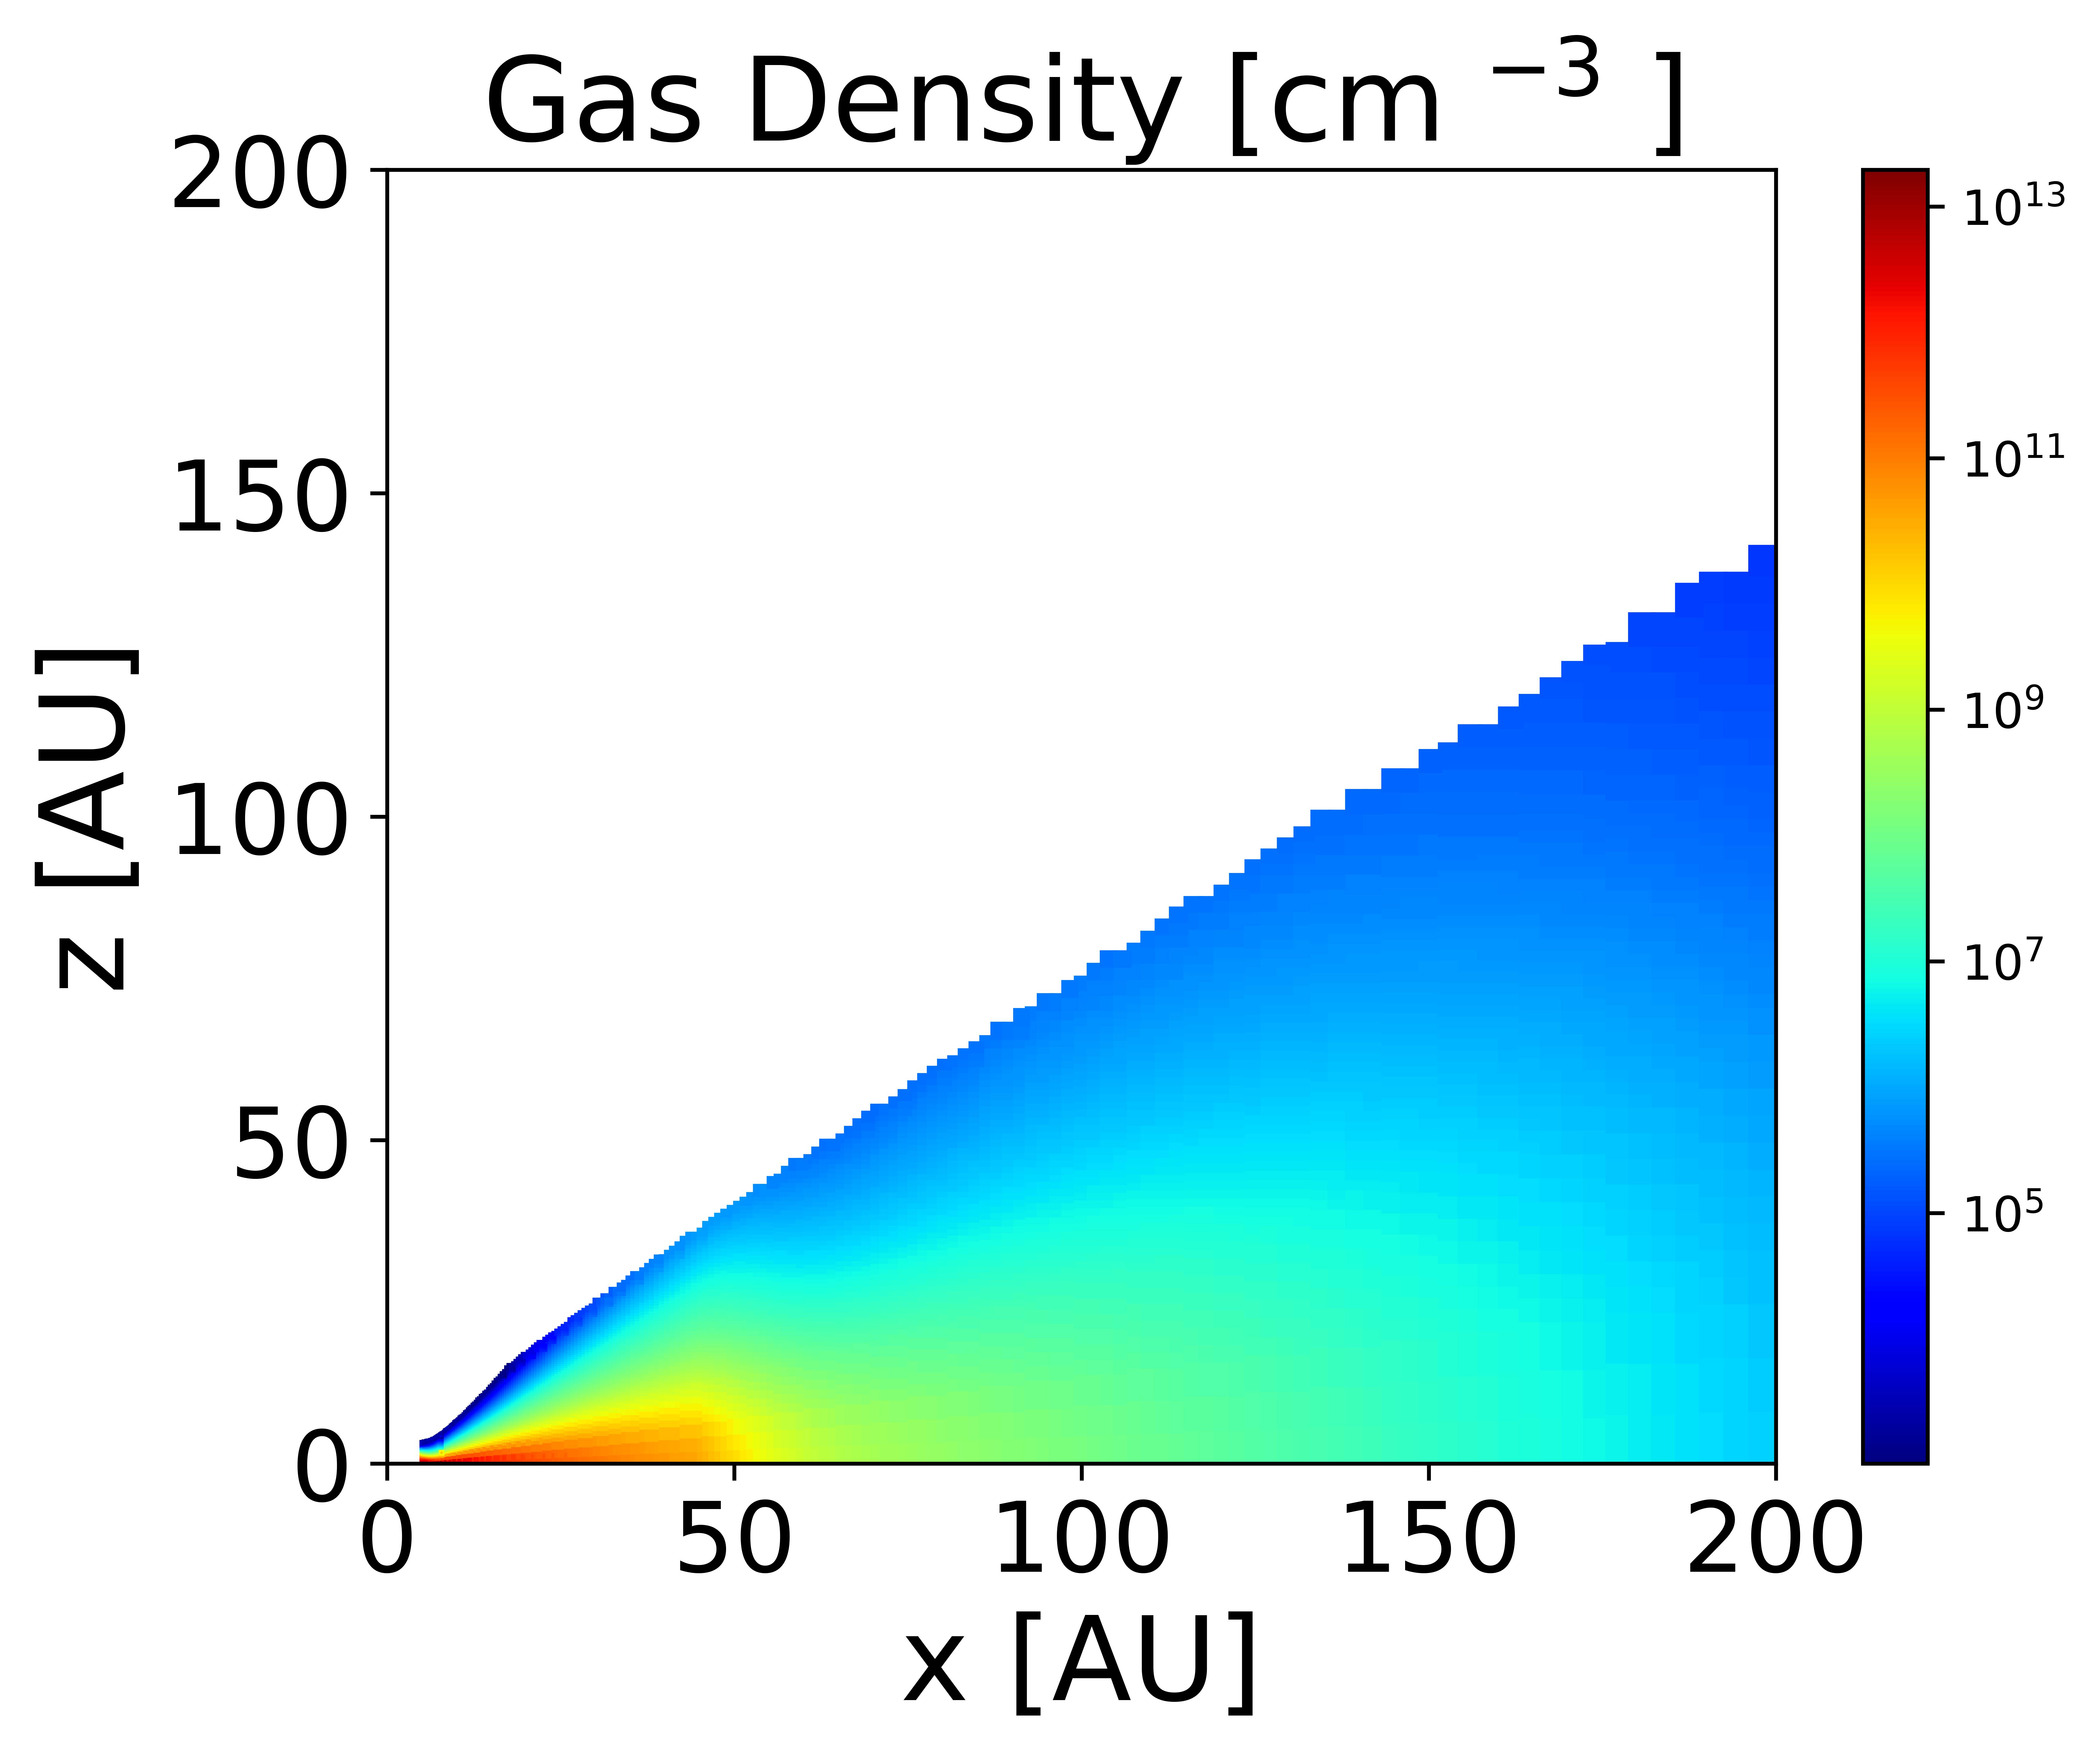
\includegraphics[width=0.6\linewidth]{n_gas}
	\caption{Parametric gas number density structure}
	\label{fig:ngas}
\end{figure}
\begin{figure}[h!]
	\centering
	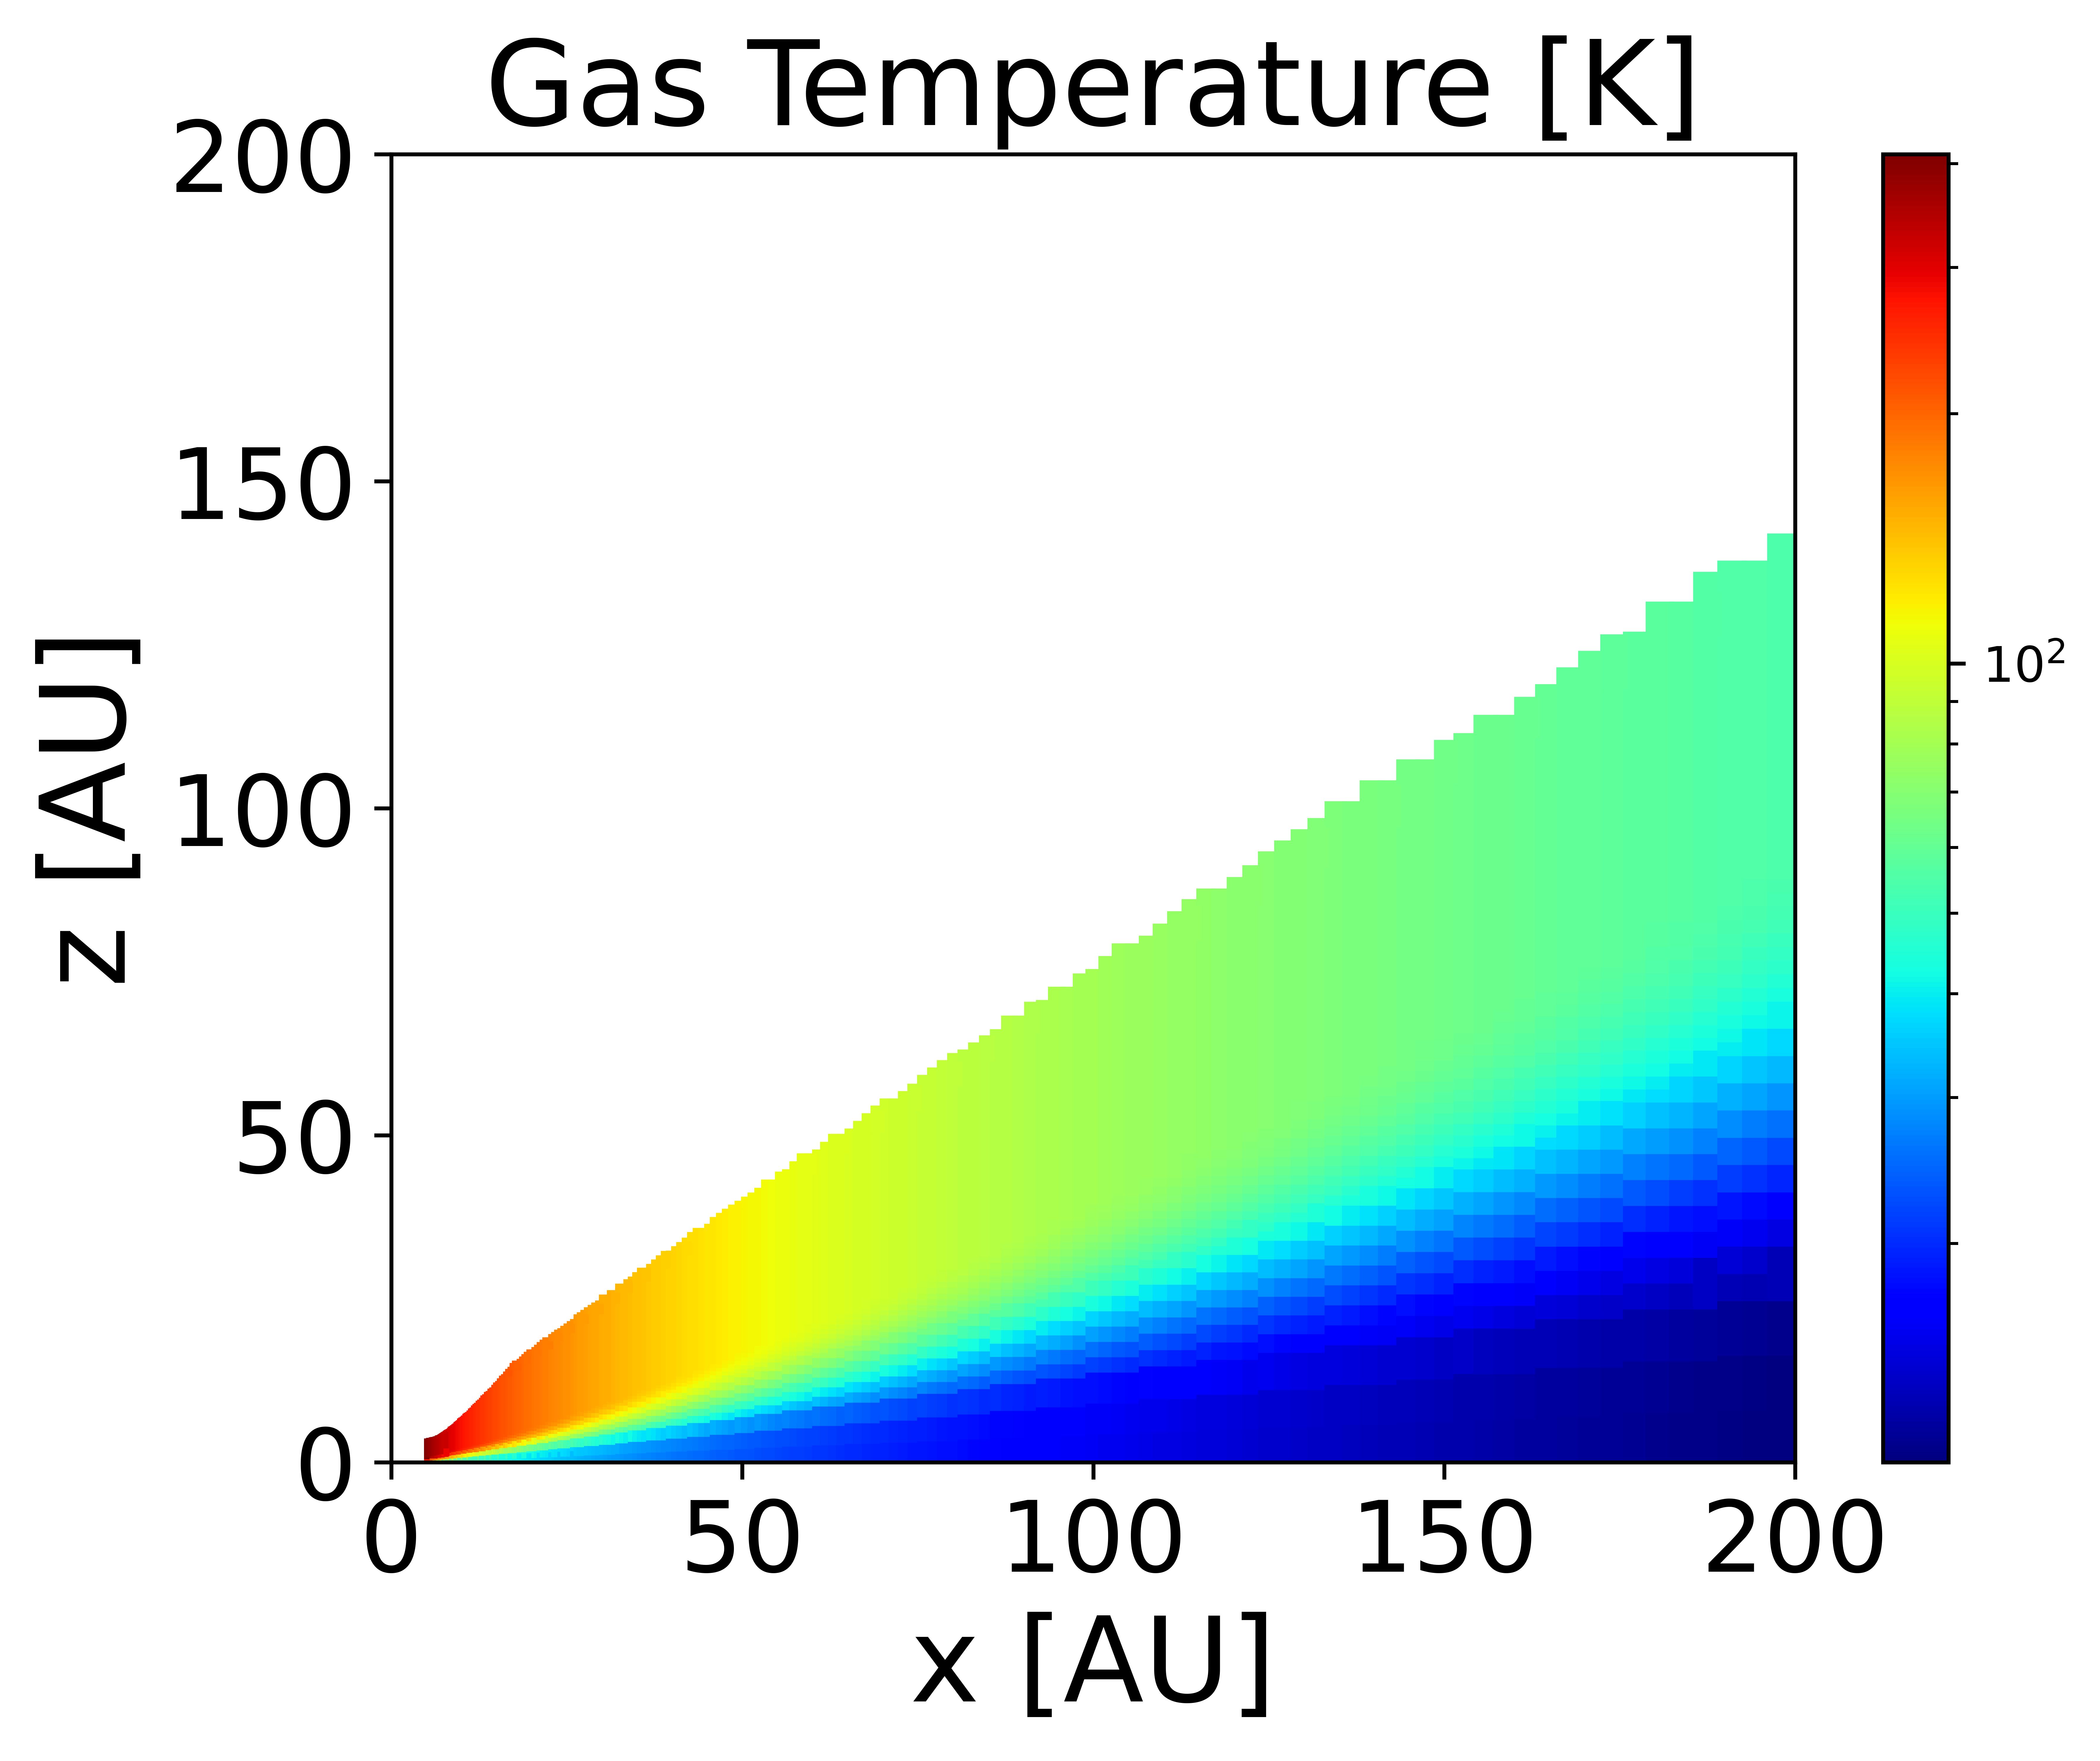
\includegraphics[width=0.6\linewidth]{Tgas}
	\caption{Parametric gas temperature structure}
	\label{fig:Tgas}
\end{figure}
\begin{figure}
	\centering
	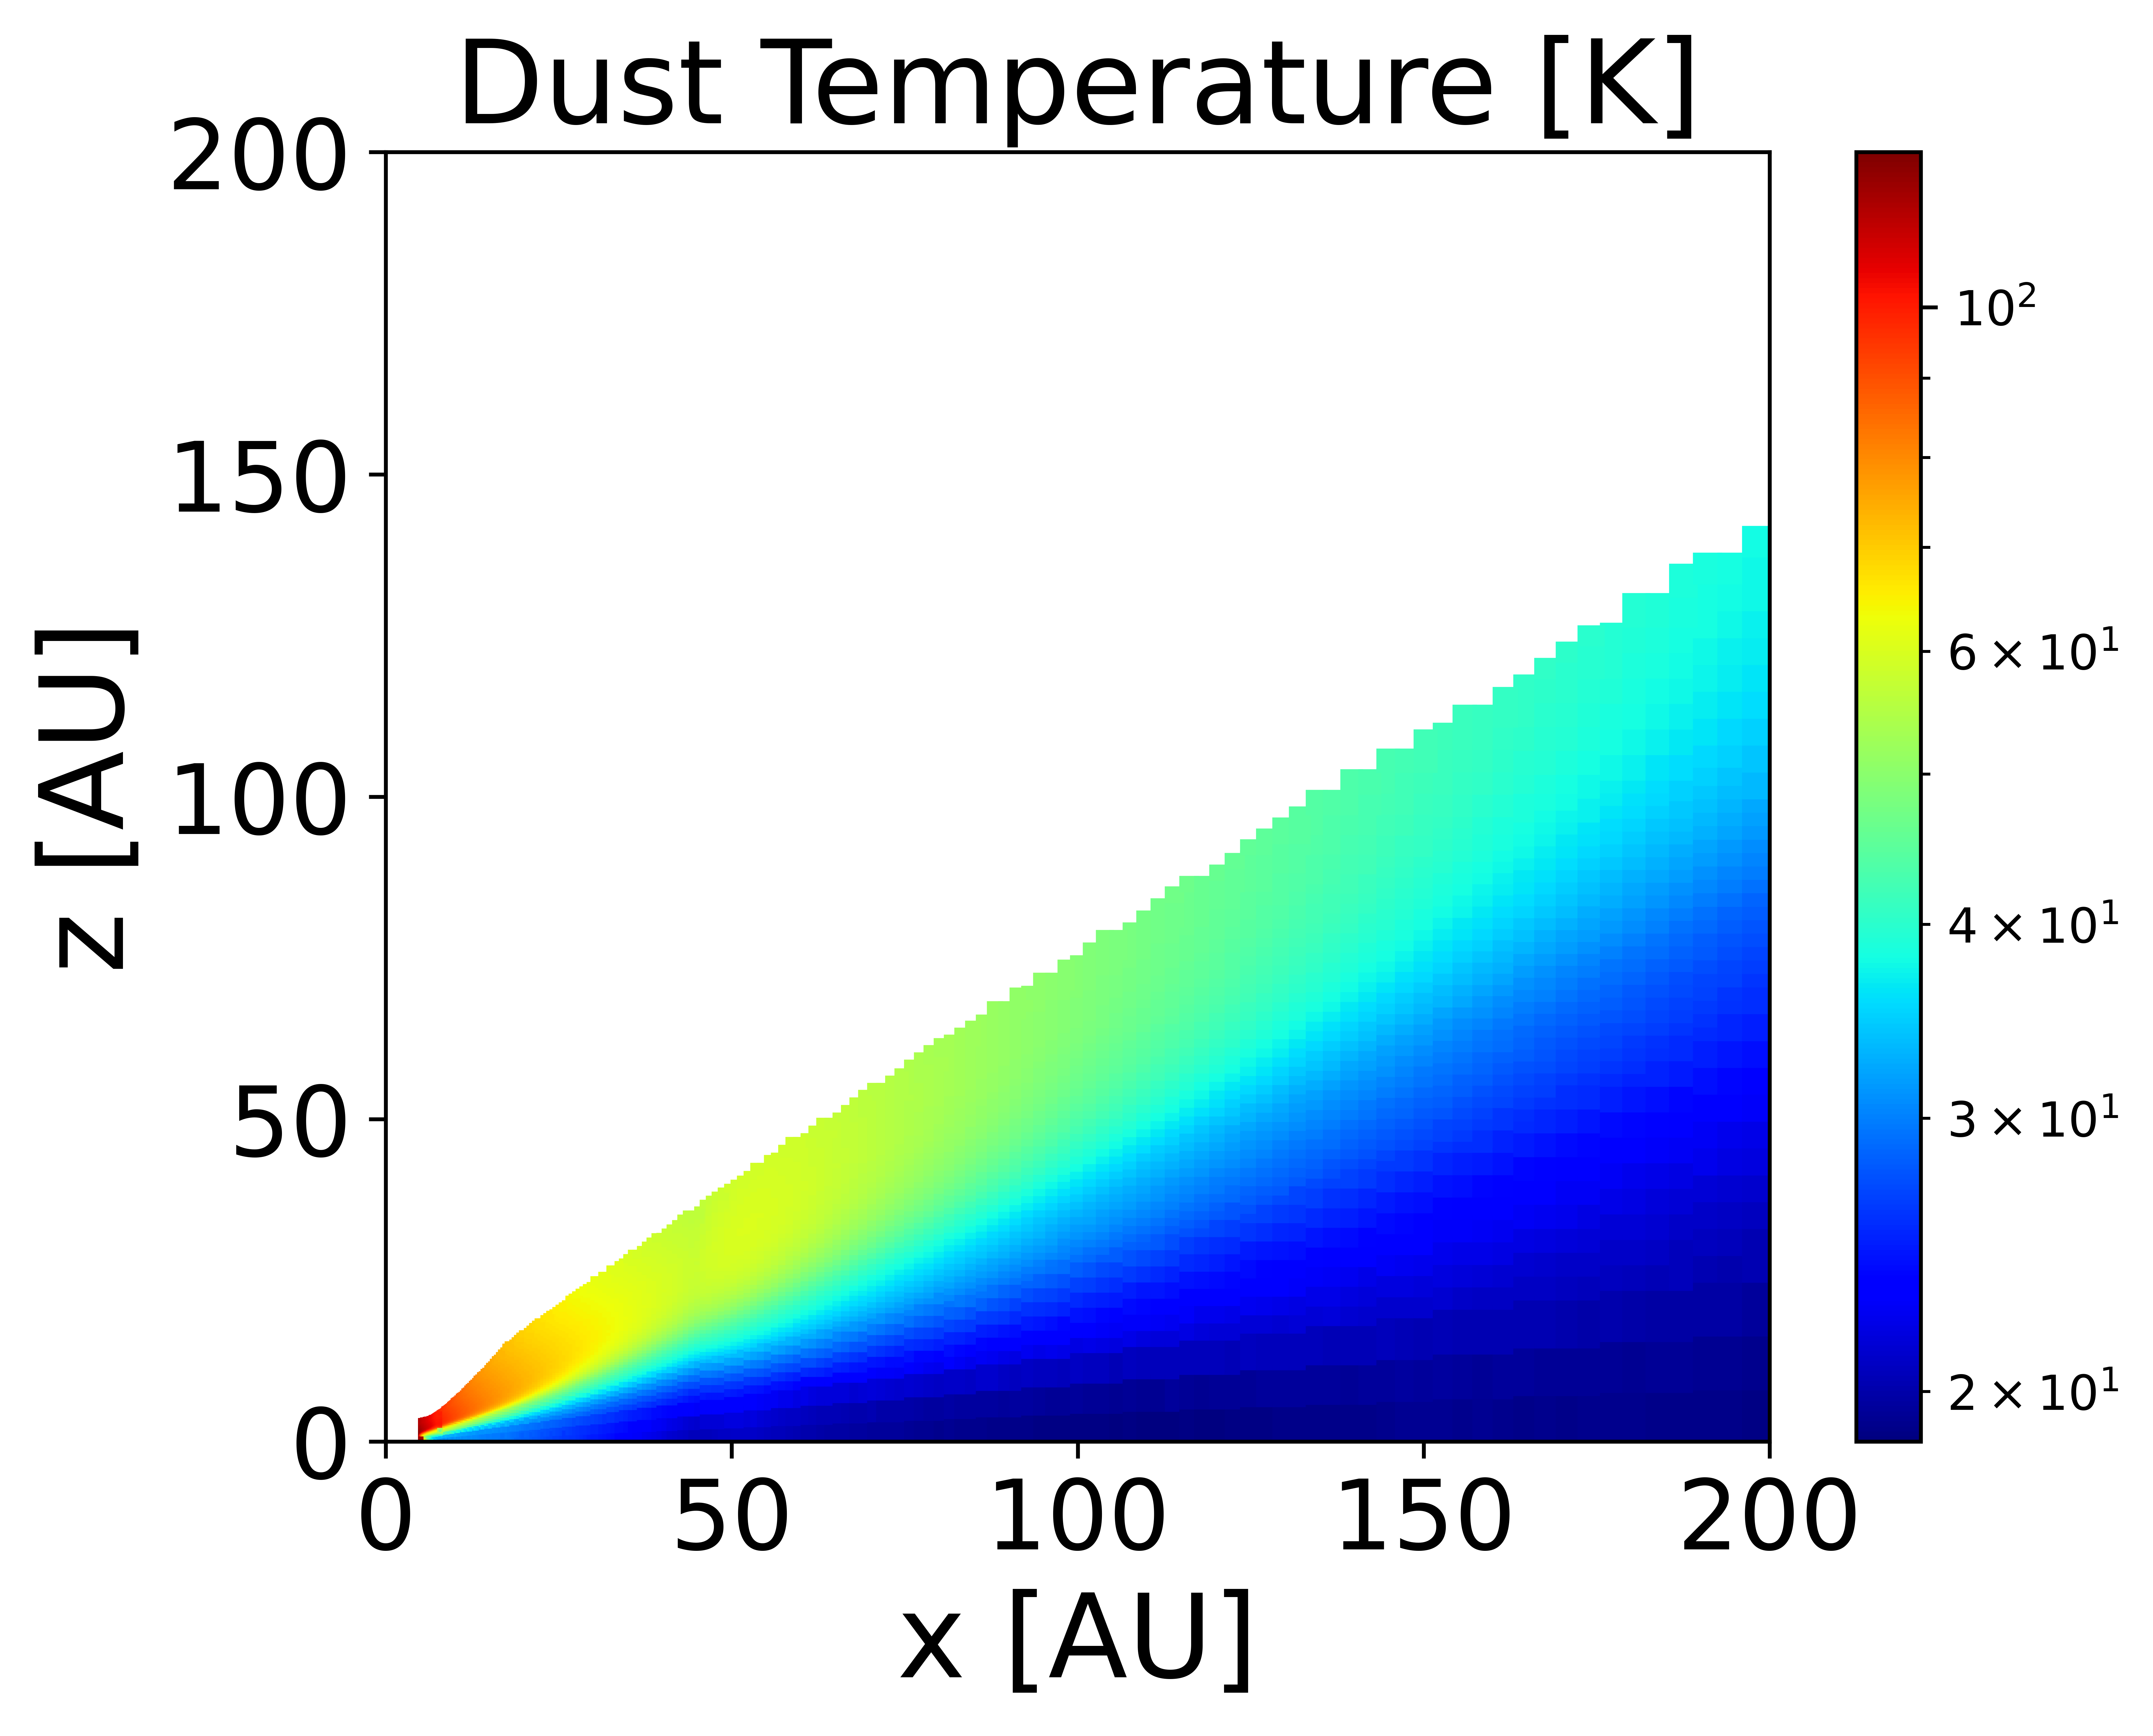
\includegraphics[width=0.6\linewidth]{Tdust}
	\caption{Dust temperature structure after dust radiative transfer}
	\label{fig:Tdust}
\end{figure}
\begin{figure}
	\centering
	\includegraphics[width=0.6\linewidth]{plot}
	\caption{Time evolution of some prominent chemical species}
	\label{fig:abun}
\end{figure}
%\begin{figure}
%	\centering
%	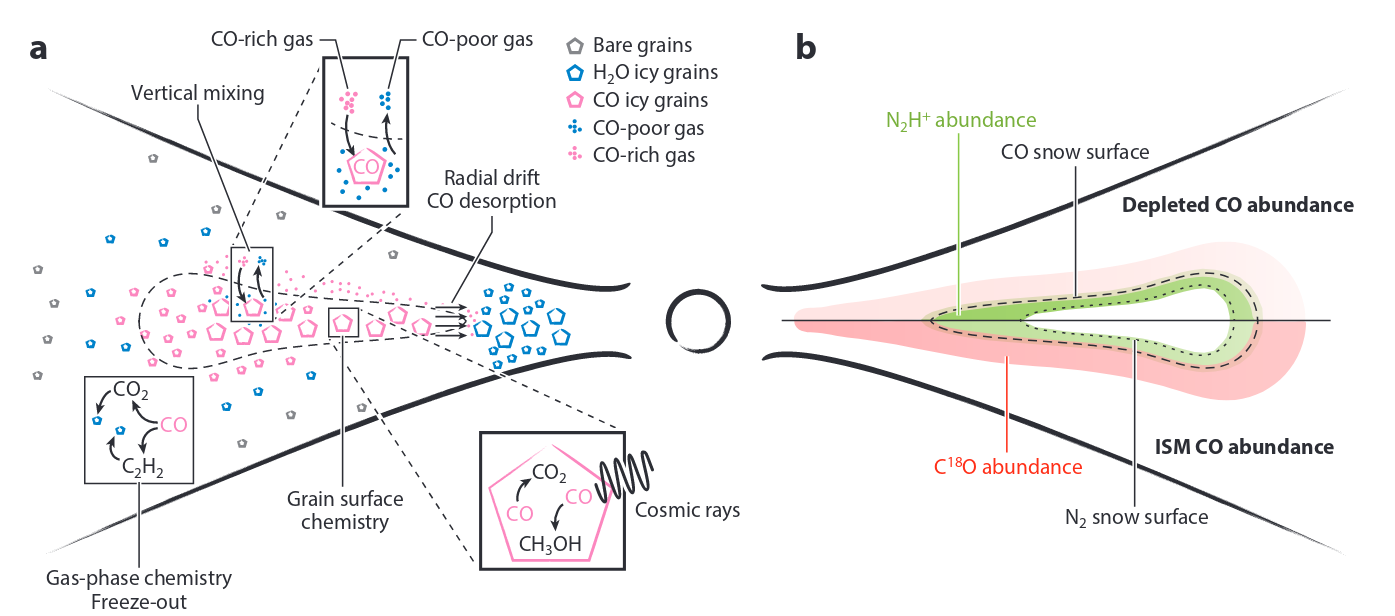
\includegraphics[width=1.1\linewidth]{screenshot003}
%	\caption{Chemically tracing disk gas content through \ce{CO} isotopologues: (a) Major physicochemical processes that reduce \ce{CO} gas abundances in protoplanetary disks, including vertical mixing and sequestration of \ce{CO} ice in the midplane, gas-phase chemistry and freeze-out, and grain surface chemistry. (b) \ce{C^{18}O} (red) and \ce{N2H^+} (green) abundances (more intense color reflects higher abundance) for depleted and interstellar medium–like \ce{CO} gas abundances.}
%	\label{fig:screenshot003}
%\end{figure}




 
 




